\section{More on GWM Task} \label{app:dataset}
%\setcounter{figure}{0}
%\setcounter{table}{0}




\begin{table*}[t]
\small
 \setlength{\tabcolsep}{7pt}
 \centering
 \renewcommand{\arraystretch}{1}
 \setlength\tabcolsep{1pt}
    \caption{\textbf{Detailed summarization of all collected datasets in GWM.} We summarize the dataset names, tasks, action level, multi-modality, nodes, and edges in the table.}
    \label{tab:dataset_all}
    \centering
    \begin{tabular}{l|ccccc}
        \toprule
        \textbf{Dataset}  & \textbf{Task} & \textbf{Action Level} &  \textbf{Multi-modality} & \textbf{Nodes} & \textbf{Edges}    \\ \midrule
        Goodreads & Multi-modal generation/matching & Node level & Text/image & Text/image nodes &  Similar-book semantic   \\
        Multi-Modal-Paper & Multi-modal generation/matching & Node level & Text/image/table & Text/image/table nodes & References \\
        Baby & Recommendation & Link level & Text/table/image & User/item nodes & User-item interactions  \\
        Sports & Recommendation & Link level & Text/table/image & User/item nodes & User-item interactions  \\
        Clothing & Recommendation & Link level & Text/table/image & User/item nodes & User-item interactions  \\
        Cora & Traditional graph prediction  & Node/edge level & Text & Research paper nodes & Citation  \\
        PubMed & Traditional graph prediction  & Node/edge level & Text & Research paper nodes & Citation  \\
        HIV & Traditional graph prediction & Graph level & Text & Atoms nodes & Atoms bonds \\
        AgentClinic&  Multi-agent collaboration  & Graph level & Text/image & Agent/image/text nodes& Agent-agent/image/text \\
        LongBench v2& Retrieval-augmented generation & Unintended action  & Text & Chunk nodes& Chunk-chunk similarity \\
        ALFWorld& Planning and optimization & Graph level & Text/image & State  nodes &  State images similarity \\ 
        \bottomrule
    \end{tabular}
% }

\end{table*}


This section discusses the detailed processing procedure for each dataset collected in GWM. We summarize their general information in Table \ref{tab:dataset_all}.

\subsection{Multi-modal generation and matching} \label{ap:multi-modal generation and matching g}

\xhdr{Dataset descriptions} In this study, we utilize two datasets for multi-modal generation and matching: the Goodreads dataset \cite{wan-etal-2019-fine} and our curated Multi-Modal-Paper dataset. 

\textbf{(1) Goodreads}: The Goodreads dataset is a large-scale collection of book-related metadata, textual descriptions, and cover images, widely used in prior multi-modal research~\cite{jin2024instructg2i}. 
The Goodreads dataset is structured as a graph, where each book is represented as a node, and edges signify similar-book semantics.

\textbf{(2) Multi-Model-Paper}: Multi-Modal-Paper dataset is a curated dataset of academic papers, incorporating textual content, figures, tables, and metadata to facilitate research on scholarly document analysis. The raw LaTeX files of the papers were collected from ArXiv\footnote{\href{https://arxiv.org/}{https://arxiv.org/} We thank ArXiv for providing open access interoperability.} using the ArXiv API, in accordance with the papers' licenses, which are primarily CC0 or CC-BY 4.0, permitting redistribution and sharing. Using carefully selected survey papers from various domains of Artificial Intelligence (AI), including Natural Language Processing (NLP), Computer Vision (CV), Bio-informatics, and Robotics, as seed papers, we employ a breadth-first search (BFS) algorithm to gather cited papers. Then, we traverse through the abstract syntax tree built from the LaTeX file to extract graph-structured multi-modal data for each gathered paper. 

For the multi-modal generation task, we sample figure-caption pairs for training and evaluation. GWM and baseline models are tasked with reconstructing the figures from the provided captions. For the multi-modal matching task, we sample cited-citing pairs using reference relationship, namely the macro command "$\backslash$ref". The cited-citing pairs are usually figure-text or table-text pairs.

A detailed statistical overview of the Goodreads and Multi-Modal-Paper datasets is presented in Table~\ref{tab:multimodal_data}.

% Todo: Statistic of the dataset
\begin{table}[ht]
	\centering
    \caption{\textbf{Data statistics for multi-modal generation and matching.} In Multi-Modal-Paper, there are 58565 text-nodes, 7380 figure-nodes, and 6792 table-nodes.}
	\begin{tabular}{lrrr}
		\toprule
		\textbf{Dataset} & \textbf{\#Node} & \textbf{\#Edges} \\
		\midrule
		\textbf{Goodreads} &  93,475 & 637,210\\
		\textbf{Multi-Modal-Paper} & 72,737 &51,840\\
		\bottomrule
	\end{tabular}
	\label{tab:multimodal_data}%
\end{table}

\xhdr{Baselines details}
For multi-modal generation tasks, we employ two text-to-image baseline models, SD-1.5 and SD-1.5 FT, along with an image-to-image baseline model, ControlNet.


 \begin{itemize}[leftmargin=1em, itemsep=0pt] 
 \item \textbf{SD-1.5}: A pre-trained Stable Diffusion v1.5 model~\cite{rombach2022high} used for text-to-image generation without task-specific fine-tuning.
\item  \textbf{SD-1.5 FT}: Stable Diffusion v1.5 models, each fine-tuned separately on the training splits of the Goodreads and Multi-Modal-Paper datasets.
\item \textbf{ControlNet}: An extension of Stable Diffusion that incorporates structural guidance, such as edge maps or depth maps, to enhance control over generated images~\cite{zhang2023adding}.
 \end{itemize} 

We use three baselines for multi-modal matching: Contrastive MLP, CLIP, and CLIP FT. Since the vertices of the edge in the Multi-Modal-Paper dataset can include tables, namely the text-table pair that are not suitable for the CLIP model, we exclusively use Contrastive MLP for this dataset.
 \begin{itemize}[leftmargin=1em, itemsep=0pt] 
 \item \textbf{Contrastive MLP} \citep{liu2022mlp}: A multi-layer perceptron trained to predict multi-modal matching by processing embeddings from different modalities. The text and table embeddings are encoded by BERT while the image embedding is encoded by CLIP. Embeddings from different modalities are padding to the same dimension.
\item  \textbf{CLIP}: A pre-trained vision-language model designed for image-text alignment, using contrastive learning to map corresponding image and text embeddings into a shared space~\cite{radford2021learning}.
\item \textbf{CLIP FT}: A fine-tuned version of CLIP, adapted to the specific dataset to enhance multi-modal matching performance.
 \end{itemize} 


\subsection{Recommendation} \label{apd:rec}

\begin{table}[ht]
	\centering
    \caption{\textbf{Data statistics for recommendation.} It includes three datasets of different scales, with the sizes ranging from small to large as follows: Baby, Sports, and Clothing.}
	\begin{tabular}{lrrrr}
		\toprule
		\textbf{Dataset} & \textbf{\#User} & \textbf{\#Item} & \textbf{\#Edges} & \textbf{Sparsity}\\
		\midrule
		\textbf{Baby} & 19,445 & 7,050 & 160,792  & 99.883\% \\
		\textbf{Sports} & 35,598 & 18,357 & 296,337  & 99.955\% \\
		\textbf{Clothing} & 39,387 & 23,033 & 278,677  & 99.969\% \\
		\bottomrule
	\end{tabular}
	\label{tab:rec_data}%
\end{table}

\xhdr{Dataset descriptions} In the recommendation task, we conduct extensive evaluations using three Amazon datasets extensively recognized in prior research~\citep{mcauley2015image}, specifically: Baby, Sports, and Outdoors, as well as Clothing Shoes, and Jewelry. For simplicity, these datasets are hereafter referred to as Baby, Sports, and Clothing, respectively. Utilizing the 5-core setting, we filter inactive users and items with less than five interactions. Each dataset encompasses both visual and textual modalities and we use the extracted visual and textual features from existing work~\citep{zhou2023mmrec}. Here the visual modality is the product image and the textual modality is the product description. The characteristics of these datasets are shown in Table~\ref{tab:rec_data}.


\xhdr{Baselines details} We compare GWM with three representative GNN baselines.

 \begin{itemize}[leftmargin=1em, itemsep=0pt] 
 \item \textbf{LightGCN}: Employs a simplified graph convolutional network to learn user and item interaction graph~\citep{lightgcn}.
\item  \textbf{MMGCN}: Learns user preferences across multiple modalities via message-passing on modality-specific user-item graphs, improving recommendations in multimedia contexts~\citep{mmgcn}.

\item \textbf{GRCN}: Refines interaction graphs using multimedia content to identify and remove noisy edges, thereby sharpening the recommendation process~\citep{grcn}.

 \end{itemize} 
 






\subsection{Traditional graph prediction} \label{apd:graph}
\xhdr{Dataset descriptions} In the traditional graph prediction task, we evaluate GWM on Cora, PubMed, and HIV datasets.
(1) Cora~\cite{chen2024exploring}: Cora is a citation network in the computer science domain, where nodes represent research papers and edges denote citation relationships. Each node includes the paper's title and abstract as text features, with labels indicating paper categories. Tasks on Cora include category prediction (node level) and citation link identification (link level).
(2) PubMed~\cite{chen2024exploring}: PubMed is a biomedical citation network, similar to Cora, with nodes representing papers and edges indicating citation relationships.
(3) HIV~\cite{liu2023one}: HIV is a molecular dataset constructed from MOLHIV dataset~\cite{wu2018moleculenet} that contains over 40,000 compounds annotated for their ability to inhibit HIV replication. Molecular structures and graph representations are generated from SMILES strings, with atoms (nodes) and bonds (edges) described using natural language.

\xhdr{Baselines details} The settings for the baselines primarily follow LLAGA \citep{chen2024llaga} and OFA \citep{liu2023one}. We convert all nodes and labels in the Cora, PubMed, and HIV datasets into text. For all methods, we use BERT to obtain text embedding. We divide all datasets into training, validation, and test sets in an 8:1:1 ratio. 

 \begin{itemize}[leftmargin=1em, itemsep=0pt] 
 \item \textbf{GCN} ~\cite{Thomas2017GCN}: Applies spectral-based convolution operations to capture local graph structures and propagate information across nodes, serving as a fundamental baseline for graph-based learning.
\item  \textbf{GAT} ~\cite{velivckovic2017gat}: Enhances node representation learning by incorporating attention mechanisms, allowing adaptive weighting of neighboring nodes to improve feature aggregation.
\item \textbf{LLAGA} ~\cite{chen2024llaga}: Integrates LLM with graph structures to enhance reasoning and information retrieval in multi-modal and structured data scenarios.
\item \textbf{OFA} ~\cite{liu2023one}: Unifies vision, language, and multi-modal learning tasks within a single framework, leveraging pre-trained knowledge to facilitate cross-modal understanding and adaptation.
 \end{itemize} 

 
\subsection{Multi-agent collaboration} \label{apd:agent}

\xhdr{Dataset descriptions} In the multi-agent collaboration task, we evaluate GWM on AgentClinic~\cite{schmidgall2024agentclinic} benchmark, specifically AgentClinic-NEJM collected from the New England Journal of Medicine (NEJM) case challenges. Each case in AgentClinic-NEJM is multimodal, comprising a case description, patient profile, clinical photograph, measurement results, and five candidate diagnoses. We partition AgentClinic-NEJM into training, validation, and test sets using a 4:1:1 split ratio. To simulate real-world clinical procedures, we employ the simulated clinical environments from AgentClinic to gather dialogues between the patient and doctor, along with physical examination results. This environment is modeled as a graph, where nodes represent various profile-based agents and edges capture the interactions between agents and their engagement with knowledge resources. We utilize Meta-Llama-3-70B-Instruct\footnote{\href{https://huggingface.co/meta-llama/Meta-Llama-3-70B-Instruct}{https://huggingface.co/meta-llama/Meta-Llama-3-70B-Instruct}} as backbone model for simulation. In the final diagnosis procedure, we apply both GWM and LLM baselines for comparison, where the graph information is converted into textual format before being processed by LLM baselines.

\xhdr{Baselines details} We compare GWM with three classic LLM baselines adopting different reasoning strategies. We use Meta-Llama-3-8B-Instruct\footnote{\href{https://huggingface.co/meta-llama/Meta-Llama-3-8B-Instruct}{https://huggingface.co/meta-llama/Meta-Llama-3-8B-Instruct}} as the backbone model to align with GWM.
 \begin{itemize}[leftmargin=1em, itemsep=0pt] 
 \item \textbf{CoT}: Adopts Chain-of-Thought~\cite{wei2022chain} prompting, which enhances reasoning by decomposing complex problems into intermediate steps, improving performance on multi-step reasoning tasks.
\item  \textbf{ToT}: Adopts Tree-of-Thought~\cite{yao2024tree} prompting, which explores multiple reasoning paths in a tree-like structure, enabling iterative evaluation and refinement for more robust decision-making.
\item \textbf{Few-shots}: Adopts Few-shot~\cite{brown2020languagemodelsfewshotlearners} prompting, where the model is provided with a limited number of in-context examples to guide task-specific reasoning without requiring fine-tuning.
 \end{itemize}


\subsection{Retrieval-augmented generation} \label{apd:RAG}

The purpose of Retrieval-Augmented Generation (RAG) is to enhance the generation capabilities of Large Language Models (LLMs) by retrieving information from external knowledge \citep{lewis2020retrieval,gao2023retrieval,zhao2024retrieval}. We introduce its dataset and baselines as follows:


\xhdr{Dataset descriptions} We employ LongBench v2 \citep{bai2024longbench}, a benchmark specifically designed to test long-context understanding and reasoning. This benchmark comprises 503 challenging multiple-choice questions, with contextual lengths ranging from 8,000 to 2 million words, spanning six major task categories: Single-Doc QA, Multi-Doc QA, Long In-context Learning, Long-dialogue History Understanding, Code Repository Understanding, and Long Structured Data Understanding. The questions are stratified into easy and hard levels based on the difficulty encountered by human experts and models during their resolution. In alignment with methodologies from previous studies such as GraphRAG \citep{edge2024local}, we segment long contexts into chunks that serve as graph nodes, with edges defined by the similarity of their BERT embeddings. Building on this, we select the Top-k (k=5 in our setting) chunks with the highest similarity to the question's embedding to feed into the GWM. For this task, we divided the dataset into training, validation, and test sets in an 8:1:1 ratio.

\xhdr{Baselines details} We conduct comparisons with two RAG-based baselines—BM25 \citep{robertson2009probabilistic} and Dragon \citep{lin2023train}—and three long-context LLMs ($128k$), including Mistral Large 2\footnote{\href{https://huggingface.co/mistralai/Mistral-Large-Instruct-2407}{https://huggingface.co/mistralai/Mistral-Large-Instruct-2407}}, Command R+\footnote{\href{https://huggingface.co/CohereForAI/c4ai-command-r-plus}{https://huggingface.co/CohereForAI/c4ai-command-r-plus}}, and GPT-4o mini\footnote{\href{https://openai.com/index/gpt-4o-mini-advancing-cost-efficient-intelligence/}{https://openai.com/index/gpt-4o-mini-advancing-cost-efficient-intelligence/}}. Their details are as follows:

 \begin{itemize}[leftmargin=1em, itemsep=0pt] 
 
\item \textbf{BM25}:  A widely-used ranking function in information sparse retrieval. It inputs the retrieved context along with the question into the Llama-3-8B model to generate a response.

\item  \textbf{Dragon}: It employs contrastive learning and other training tricks to finetune its ability to retrieve memory chunks. Using the Llama-3-8B model, it processes the retrieved context and the question to produce a response.

\item \textbf{Mistral Large 2}: Mistral Large 2 from Mistral AI boasts 123 billion parameters, with a context limit of 128 k tokens. This model is one of the largest currently available, offering exceptional depth in language understanding and generation capabilities, suited for tackling the most demanding NLP tasks across various domains. 

\item \textbf{Command R+}: Command R+ by Cohere is a massive language model with 104 billion parameters, also supporting a context size of up to 128 k tokens. It is optimized for understanding and executing complex commands, making it particularly effective in interactive applications where precise and nuanced language comprehension is critical.
 
\item  \textbf{GPT-4o mini}: GPT-4o mini, developed by OpenAI, is a variant of the GPT-4 series. Unlike its larger counterparts, specific details about the model's size in terms of parameters are not provided, but it is designed to handle a maximum context size of 128k tokens. This model is geared towards applications requiring high-quality text generation with potentially limited computational resources.

\end{itemize}



\subsection{Planning and optimization} \label{apd:opt}

This task is designed to measure how effectively different methods can imitate the trajectory of expert strategies, which is very helpful for planning and optimization tasks.

\xhdr{Dataset descriptions} We employ the expert strategy dataset from the text-based embodied task framework, ALFWorld \citep{shridhar2020alfworld,yang2024embodied}. This dataset provides detailed descriptions of the expert's strategic state at each decision point, incorporating both images and text, along with the corresponding decisions made in text format. In our approach, we represent each decision state as nodes within a graph and establish edges between these nodes based on the similarity of the state images linked to each decision. Our total sample size is 10,000, and it is divided into training, validation, and test sets in an 8:1:1 ratio.

\xhdr{Baselines details} For all baselines, we first use LLaVA-1.5-7B to convert the image of each state into a text description. 

 \begin{itemize}[leftmargin=1em, itemsep=0pt] 
 \item \textbf{Normal}: It directly inputs the text description of the current state into Llama-3-8B to get the response.  
 
\item  \textbf{COT}: It adopts Chain-of-Thought~\cite{wei2022chain} prompting into baseline Normal to enhance reasoning ability when predicting.

\item \textbf{T5 FT \citep{raffel2020exploring}}:  It is a versatile language model designed by Google Research, which treats every language problem as a text-to-text task, enhancing its adaptability across a broad range of NLP applications. Here we finetune it on the dataset of this task.

 \end{itemize}




\section{Hyper-parameters} \label{sec:hyper}

For the GWM-E, we employ an n-hop MLP, where for the LLM decoder each MLP has dimensions of 2048*4096, and for the SD decoder, each MLP has dimensions of 2048*768. We fix the parameters of LLM and only fine-tune the parameters of MLP. For GWM-T, we select a maximum of 2k token-limited hops for each task to ensure a balance between efficiency and performance. We apply Lora (Lora rank = 8) \citep{hu2021lora} for efficient training. We have summarized the hyperparameters for training different models in Table \ref{apx:tab:hyper}.



\begin{table}[ht]
\caption{Hyper-parameter configuration for model training.}\label{apx:tab:hyper}
\centering
\scalebox{0.63}{
\begin{tabular}{ccccc}
\toprule
Parameter & GWM-T LLM & GWM-T SD & GWM-E LLM & GWM-E SD \\
\midrule
Optimizer & AdamW & AdamW & AdamW & AdamW \\
% \midrule
% \midrule
Adam $\epsilon$ & 1e-8  & 1e-8 & 1e-8  & 1e-8 \\
Adam $(\beta_1, \beta_2)$ & (0.9, 0.999) & (0.9, 0.999) & (0.9, 0.999)  & (0.9, 0.999)  \\
Weight decay & 1e-2 & 1e-2 & 1e-2  & 1e-2 \\

Batch size per GPU & 4 & 1 & 10 & 16\\
Gradient Accumulation & 8 & 4 & 1 & 4\\

Epochs & 4 & 5 & 1  & 30 \\
Resolution & - & 512 & - & 256 \\
% \midrule
Learning rate & 3e-4 & 1e-5 &  3e-4  & 1e-5 \\
Backbone SD &  Llama-3-8B & SD-v1-5 &  Llama-3-8B & SD-v1-5   \\
\bottomrule            
\end{tabular}
}
\end{table}

 
\section{Prompt Usage of GWM} \label{sec:prompt}

We summarize all the prompts we used in GWM in this section. We first introduce the action prompts in GWM. Specifically, we have summarized the action prompts for multi-modal generation and matching in Tables \ref{prompt-template:multi-modal generation} and \ref{prompt-template:multi-modal matching}. The action prompts for recommendations are summarized in Table \ref{prompt-template:recommendation}. Additionally, the action prompts for traditional graph prediction are outlined in Tables \ref{prompt-template:Cora_node}, \ref{prompt-template:PubMed_node}, \ref{prompt-template:link prediction}, and \ref{prompt-template:HIV}. Moreover, we have also summarized the action prompts for multi-agent collaboration, retrieval-augmented generation, and planning and optimization in Tables \ref{prompt-template:multi-agent collaboration}, \ref{prompt-template:retrieval-augmented generation}, and \ref{prompt-template:planning and optimization}.  Then, we introduce prompts used in GWM-T. We summarize the prompt $P_{u}$ of multi-modality as tokens in GWM-T in Table \ref{prompt-template:multi-modality as token}. Moreover, we introduce the prompt $f_{v}(\cdot)$ of aggregating central node and neighbor nodes in GWM-T in Table \ref{prompt-template:aggregating}.

%\section{Additional Related Work} \label{apd:Additional Related Work}


%\xhdr{Graph for Modelling Relations} Graphs are highly effective in modeling complex relationships \citep{fey2023relational,cao2023relational,gao2020ci,chen2022gndan,wu2022graph,yang2021consisrec}, extracting nodes and edges to model relational data with embeddings. Traditional methods like label propagation \citep{xie2022graphhop,zhu2002learning} use edge relationships to spread known labels to target nodes. However, with advances in deep learning, Graph Neural Networks (GNNs) \citep{Thomas2017GCN,hamilton2017graphsage,velivckovic2017gat,schlichtkrull2017modeling} have emerged as a dominant approach, particularly in recommendation systems \citep{Erxue2022recommender} and social networks \citep{wu2020social}. To further address the vast array of tasks and data, scholars have proposed the GFM \citep{chen2024llaga,liu2023one} to explore GNNs' zero-shot or few-shot capabilities \citep{fey2023relational,cao2023relational,gao2020ci,chen2022gndan} to tackle challenges such as the cold start problem in recommendations. 




%\xhdr{World Model} The WM \citep{ha2018recurrent} is to construct the world observations as states and predict future states based on given actions. Existing WMs \citep{wu2024ivideogpt,bruce2024genie} primarily focus on how to utilize unstructured data such as sequence data to predict state transitions, thereby enhancing the effectiveness of sequence generation tasks. For example, Genie \citep{bruce2024genie} trained a foundation world model using a massive amount of unlabelled, serialized internet videos, which has provided benefits for the planning outcomes of downstream tasks. Additionally, in recent years, some WMs \citep{zhang2021world,zhu2022value} have attempted to integrate structured data with GWM. For instance, $L^3P$ \citep{zhang2021world} uses graphs to model each step of the agent's decision-making process and their connections, thus enhancing scalable planning in reinforcement learning. However, they are still largely confined to planning and optimization scenarios, which limits their potential for task generalization as WMs. Therefore, by deeply integrating the capabilities of graphs with WM, we have developed GWM, which can generalize across diverse tasks such as world prediction, generation, and planning.


\begin{table*}[h]
\centering
\caption{\textbf{Action prompt of multi-modal generation}.}
\begin{tabular}{p{13cm}}
\toprule[1.1pt]
    This is a multi-modal generation task. Please predict the missing modality based on the given modality: \{modality\}.\\
\bottomrule[1.1pt]
\label{prompt-template:multi-modal generation}
\end{tabular}
\end{table*}



\begin{table*}[h]
\centering
\caption{\textbf{Action prompt of multi-modal matching}.}
\begin{tabular}{p{13cm}}
\toprule[1.1pt]
    This task involves matching multi-modal information. Given two modalities: \{modality 1\} and \{modality 2\}, please determine whether they correspond with each other. \\
\bottomrule[1.1pt]
\label{prompt-template:multi-modal matching}
\end{tabular}
\end{table*}




\begin{table*}[h]
\centering
\caption{\textbf{Action prompt of recommendation}.}
\begin{tabular}{p{13cm}}
\toprule[1.1pt]
    This is a recommendation task. Given the user node and item node: \{user node\} and \{item node\}, please tell me whether these two nodes should connect to each other.\\
\bottomrule[1.1pt]
\label{prompt-template:recommendation}
\end{tabular}
\end{table*}


\begin{table*}[h]
\centering
\caption{\textbf{Action prompt of node classification of Cora}.}
\begin{tabular}{p{13cm}}
\toprule[1.1pt]
    Given a node-centered graph: \{node\}, each node represents a paper, we need to classify the center node into 7 classes: Case Based, Genetic Algorithms, Neural Networks, Probabilistic Methods, Reinforcement Learning, Rule Learning, Theory, please tell me which class the center node belongs to?\\
\bottomrule[1.1pt]
\label{prompt-template:Cora_node}
\end{tabular}
\end{table*}

\begin{table*}[h]
\centering
\caption{\textbf{Action prompt of node classification of PubMed}.}
\begin{tabular}{p{13cm}}
\toprule[1.1pt]
    Given a node-centered graph: \{node\}, each node represents a paper about Diabetes, we need to classify the center node into 3 classes: Diabetes Mellitus Experimental, Diabetes Mellitus Type 1, and Diabetes Mellitus Type 2, please tell me which class the center node belongs to?\\
\bottomrule[1.1pt]
\label{prompt-template:PubMed_node}
\end{tabular}
\end{table*}

\begin{table*}[h]
\centering
\caption{\textbf{Action prompt of link prediction of  Cora and PubMed}.}
\begin{tabular}{p{13cm}}
\toprule[1.1pt]
    Given two nodes information: \{node 1\} and \{node 2\}, please tell me whether two center nodes in the subgraphs should connect to each other. \\
\bottomrule[1.1pt]
\label{prompt-template:link prediction}
\end{tabular}
\end{table*}

\begin{table*}[h]
\centering
\caption{\textbf{Action prompt of graph classification of  HIV}.}
\begin{tabular}{p{13cm}}
\toprule[1.1pt]
    Human immunodeficiency viruses (HIV) are a type of retrovirus, which induces acquired immune deficiency syndrome (AIDs). Please determine whether this molecule \{molecule\} is effective for this assay. \\
\bottomrule[1.1pt]
\label{prompt-template:HIV}
\end{tabular}
\end{table*}



\begin{table*}[h]
\centering
\caption{\textbf{Action prompt of multi-agent collaboration}.}
\begin{tabular}{p{13cm}}
\toprule[1.1pt]
    This is a Multi-Agent Collaborative Generation task for creating dynamic conversational interactions. Given a user query: \{user query\} and context of three distinct agents: \{Patient Agent Context\}, \{Measurement Agent Context\}, and \{Moderato Agent Context\}, Please generate a well-rounded response to the user's question.\\
\bottomrule[1.1pt]
\label{prompt-template:multi-agent collaboration}
\end{tabular}
\end{table*}

\begin{table*}[h]
\centering
\caption{\textbf{Action prompt of retrieval-augmented generation}.}
\begin{tabular}{p{13cm}}
\toprule[1.1pt]
    This is a Retrieval-Augmented Generation task for improving response quality in dialogue systems. Given a user query: \{user query\} and a set of retrieved documents: \{retrieved documents\}, the goal is to generate a coherent and contextually relevant response. Please generate a response that integrates information from the retrieved documents to accurately address the user's query. \\
\bottomrule[1.1pt]
\label{prompt-template:retrieval-augmented generation}
\end{tabular}
\end{table*}

\begin{table*}[h]
\centering
\caption{\textbf{Action prompt of planning and optimization}.}
\begin{tabular}{p{13cm}}
\toprule[1.1pt]
    This is an embodied household task, please predict the next decision-making behavior based on multimodal historical information: \{historical information\}. \\
\bottomrule[1.1pt]
\label{prompt-template:planning and optimization}
\end{tabular}
\end{table*}

\begin{table*}[h]
\centering
\caption{\textbf{Prompt $P_{u}$ of multi-modality as token in GWM-T}.}
\begin{tabular}{p{13cm}}
\toprule[1.1pt]
    The image's text description is: \{image's text description\}, original text is: \{original text\}, table description is: \{table description\}. \\
\bottomrule[1.1pt]
\label{prompt-template:multi-modality as token}
\end{tabular}
\end{table*}


\begin{table*}[h]
\centering
\caption{\textbf{Prompt $f_{v}(\cdot)$ of aggregating central node and neighbor nodes in GWM-T}.}
\begin{tabular}{p{13cm}}
\toprule[1.1pt]
    The text description of the central node is: \{center node\}, and the text descriptions of the neighboring nodes are: \{neighbor nodes\}. \\
\bottomrule[1.1pt]
\label{prompt-template:aggregating}
\end{tabular}
\end{table*}



\section{Qualitative Comparisons for All Tasks of GWM} \label{app:Qualitative Comparisons}


These tables present comprehensive qualitative comparisons across all task categories evaluated in our GWM framework study. Each table demonstrates the superior performance of our Graph World Model (GWM) variants compared to state-of-the-art baselines through concrete examples. Table \ref{tab:multimodal_generation} showcases multi-modal generation capabilities where GWM-T successfully predicts missing modalities from given inputs. Table \ref{tab:multimodal_matching} illustrates multi-modal matching tasks where GWM-E accurately determines correspondence between different modalities. Table \ref{tab:recommendation} demonstrates recommendation performance where GWM-E correctly predicts user-item connections. Table \ref{tab:graph_prediction} highlights traditional graph prediction tasks where GWM-E excels in node classification. Table \ref{tab:multiagent_collaboration} presents multi-agent collaboration scenarios where GWM-T integrates multiple agent contexts for medical diagnosis. Table \ref{tab:rag} shows retrieval-augmented generation capabilities where GWM-E effectively combines retrieved documents with user queries. Finally, Table \ref{tab:planning_optimization} demonstrates planning and optimization tasks where GWM-E predicts optimal decision-making behaviors in embodied environments. These qualitative results consistently validate the effectiveness of our approach across diverse task domains.

\begin{table*}[h]
    \centering
    \caption{\textbf{Task description and output comparison of multi-modal generation.} This task is to predict the missing modality based on the given
modality. Here we utilize one case of Goodreads dataset as examples. We show the output results of GWM-T, the best performing GWM, and ControlNet , the strongest baseline.}
    \label{tab:multimodal_generation}
    
    \renewcommand{\arraystretch}{1.2} % Slightly increase row height
    
    \begin{tabular}{|m{3cm}|P{3cm}|P{3cm}|P{3cm}|}
        \toprule
        \multicolumn{4}{|c|}{\textbf{Task Description}} \\
        \midrule
        \centering \textbf{Task Name} & \multicolumn{3}{c|}{Multi-modal generation} \\
        \midrule
         \centering \textbf{Given modality} & \textbf{Action prompt} & \multicolumn{2}{c|}{\textbf{Ground truth}} \\
        \midrule
         \parbox{3cm}{\centering Title: The Shark-Infested Custard}& 
         \parbox{3cm}{\centering\arraybackslash This is a multi-modal generation task. Please predict the missing modality based on the given modality: \{modality\}.} & 
        \multicolumn{2}{m{4cm}|}{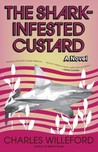
\includegraphics[width=2.8cm]{figs/Goodreads_gt_shark.jpg}} \\
        \midrule
        \centering \textbf{Method} & \multicolumn{3}{c|}{\textbf{Output Results}} \\
        \midrule
        \centering\arraybackslash
        ControlNet  & \multicolumn{3}{m{8.5cm}|}{\centering\arraybackslash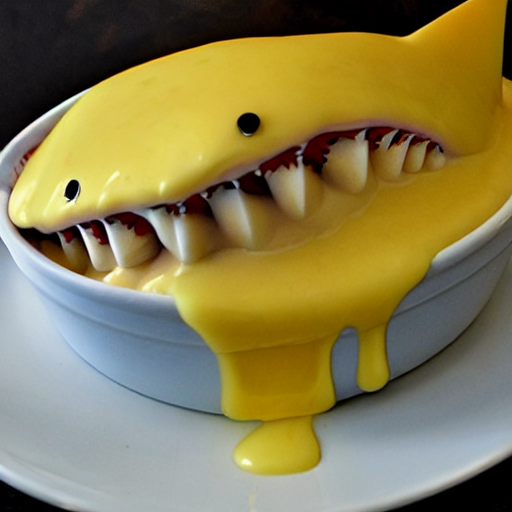
\includegraphics[width=6cm]{figs/Goodreads_controlnet_shark.png}} \\
        \midrule
        \centering\arraybackslash
        GWM-T & \multicolumn{3}{m{8.5cm}|}{\centering\arraybackslash
\includegraphics[width=6cm]{figs/Goodreads_GWMT_shark.jpg}} \\
        \bottomrule
    \end{tabular}
\end{table*}

\begin{table*}[h]
    \centering
    \caption{\textbf{Task description and output comparison of multi-modal matching.} This task is to predict whether two modalities correspond with each other. Here we utilize one case of Multi-Modal-Paper dataset as examples. We show the output results of GWM-E, the best performing GWM, and Contrastive MLP, the strongest baseline. Note that modality can be an image, a table, or a text.}
    \label{tab:multimodal_matching}
    
    \renewcommand{\arraystretch}{1.2} % Slightly increase row height
    
    % Define a new column type for centered text in m columns
    \newcolumntype{C}[1]{>{\centering\arraybackslash}m{#1}}
    
    \begin{tabular}{|C{5cm}|C{3cm}|C{5cm}|C{3cm}|C{3cm}|}
        \toprule
        \multicolumn{5}{|c|}{\textbf{Task Description}} \\
        \midrule
        \multicolumn{2}{|c|}{\textbf{Task Name}} & \multicolumn{3}{c|}{Multi-modal matching} \\
        \midrule
        \textbf{Modality 1: figure} & \textbf{Modality 2: text} & \textbf{Action prompt} & \multicolumn{2}{c|}{\textbf{Ground truth}} \\
        \midrule
        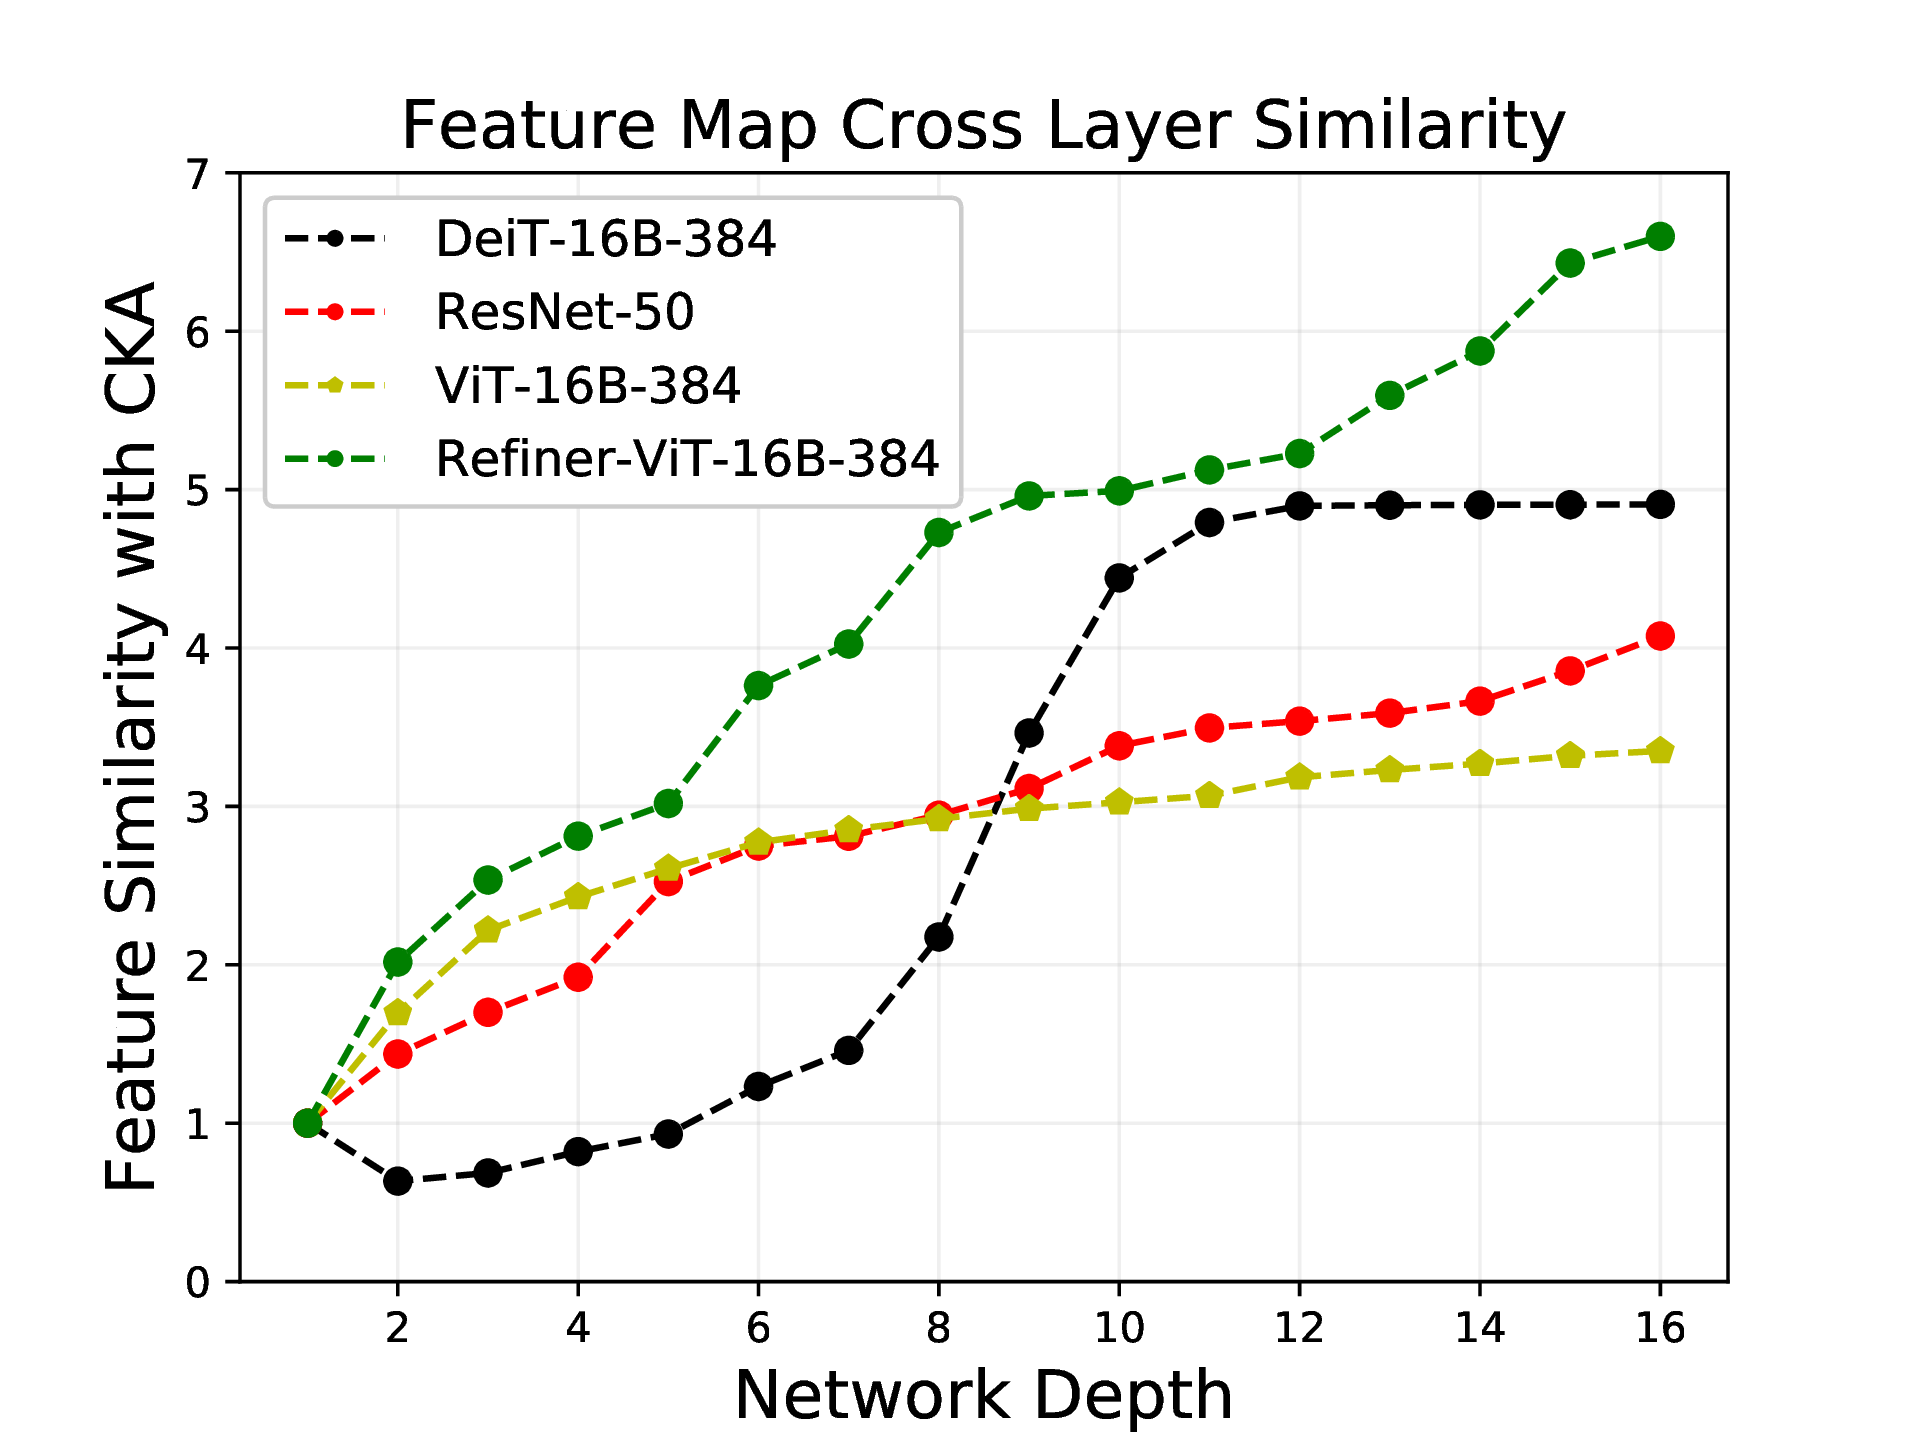
\includegraphics[width=5cm]{figs/figures_749.png} & 
        Illustration of different formats of STL expressions. (a) Different expression formats of the same STL. (b) The binary tree representation of STL. & 
        This task involves matching multi-modal information. Given two modalities: \{modality 1\} and \{modality 2\}, please determine whether they correspond with each other. & 
        \multicolumn{2}{c|}{yes} \\
        \midrule
        \multicolumn{2}{|c|}{\textbf{Method}} & \multicolumn{3}{c|}{\textbf{Output Results}} \\
        \midrule
        \multicolumn{2}{|c|}{Contrastive MLP} & \multicolumn{3}{c|}{no} \\
        \midrule
        \multicolumn{2}{|c|}{GWM-E} & \multicolumn{3}{c|}{yes} \\
        \bottomrule
    \end{tabular}
\end{table*}

\begin{table*}[h]
    \centering
    \caption{\textbf{Task description and output comparison of recommendation.} This task is to predict whether the user node and the item node are connected. Here we utilize one case of Baby dataset as examples. We show the output results of GWM-E, the best performing GWM, and LightGCN, the strongest baseline.}
    \label{tab:recommendation}
    
    \renewcommand{\arraystretch}{1.2} % Slightly increase row height
    
    % Define a new column type for centered text in m columns
    \newcolumntype{C}[1]{>{\centering\arraybackslash}m{#1}}
    
    \begin{tabular}{|C{4cm}|C{4cm}|C{4cm}|C{3cm}|C{3cm}|}
        \toprule
        \multicolumn{5}{|c|}{\textbf{Task Description}} \\
        \midrule
        \multicolumn{2}{|c|}{\textbf{Task Name}} & \multicolumn{3}{c|}{Recommendation} \\
        \midrule
        \textbf{User node} & \textbf{Item node} & \textbf{Action prompt} & \multicolumn{2}{c|}{\textbf{Ground truth}} \\
        \midrule
        User online product reviews series: I struggled to find full slips, especially larger ones. The first one was too small; the second fit well and was affordable. The beads looked stunning, perfect for beadwork. The earrings broke immediately due to poor quality. I love the 3 flower sister Hawaii glass beads on my Pandora bracelet. They're pretty and large, and my eight-year-old finds them comfy enough to sleep in ...  
          & 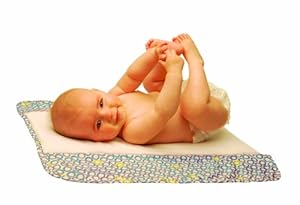
\includegraphics[width=4cm]{figs/B004R1REP2.jpg} & 
        This is a recommendation task. Given the user node and item node: \{user node\} and \{item node\}, please tell me whether these two nodes should connect to each other. & 
        \multicolumn{2}{c|}{no} \\
        \midrule
        \multicolumn{2}{|c|}{\textbf{Method}} & \multicolumn{3}{c|}{\textbf{Output Results}} \\
        \midrule
        \multicolumn{2}{|c|}{LightGCN} & \multicolumn{3}{c|}{yes} \\
        \midrule
        \multicolumn{2}{|c|}{GWM-E} & \multicolumn{3}{c|}{no} \\
        \bottomrule
    \end{tabular}
\end{table*}

\begin{table*}[h]
    \centering
    \caption{\textbf{Task description and output comparison of traditional graph prediction.} This task aims to perform predictions at three different levels: node, link, and graph. Here we utilize one case of Cora's node prediction. We show the output results of GWM-E, the best performing GWM, and LLAGA, the strongest baseline.}
    \label{tab:graph_prediction}
    
    \renewcommand{\arraystretch}{1.2} % Slightly increase row height
    
    % Define a new column type for centered text in m columns
    \newcolumntype{C}[1]{>{\centering\arraybackslash}m{#1}}
    
    \begin{tabular}{|C{7cm}|C{5cm}|C{3cm}|}
        \hline
        \multicolumn{3}{|c|}{\textbf{Task Description}} \\
        \hline
        \textbf{Task Name} & \multicolumn{2}{c|}{Traditional graph prediction} \\
        \hline
        \textbf{Node} & \textbf{Action prompt} & \textbf{Ground truth} \\
        \hline
        Learning under persistent drift: In this paper we study learning algorithms for environments which are changing over time. Unlike most previous work, we are interested in the case where the changes might be rapid but their "direction" is relatively constant. We model this type of change by assuming that the target distribution is changing continuously at a constant rate from one extreme distribution to another. We show in this case how to use a simple weighting scheme to estimate the error of an hypothesis, and using this estimate, to minimize the error of the prediction. & 
        Given a node-centered graph: \{node\}, each node represents a paper, we need to classify the center node into 7 classes: Case Based, Genetic Algorithms, Neural Networks, Probabilistic Methods, Reinforcement Learning, Rule Learning, Theory, please tell me which class the center node belongs to? & 
        Theory \\
        \hline
        \textbf{Method} & \multicolumn{2}{c|}{\textbf{Output Results}} \\
        \hline
        LLAGA & \multicolumn{2}{c|}{Neural Networks} \\
        \hline
        GWM-E & \multicolumn{2}{c|}{Theory} \\
        \hline
    \end{tabular}
\end{table*}





% \begin{table*}[h]
%     \centering
%     \caption{\textbf{Task description and output comparison of multi-agent collaboration.} The purpose of this task is to answer patients' disease-related queries based on agent-agent interaction and the interaction between the agent and external knowledge. We show the output results of GWM-T, the best performing GWM, and COT, the strongest baseline. \textbf{Please note that the image in the table may cause discomfort. We apologize for this, but these images are all sourced from real datasets.}}
%     \label{tab:multiagent_collaboration}
    
%     \renewcommand{\arraystretch}{1.1} % Slightly increase row height
    
%     \begin{tabular}{|>{\centering\arraybackslash}m{5cm}|>{\centering\arraybackslash}m{6cm}|>{\centering\arraybackslash}m{7cm}|}
%         \hline
%         \multicolumn{3}{|c|}{\textbf{Task Description}} \\
%         \hline
%         \multicolumn{1}{|c|}{\textbf{Task Name}} & \multicolumn{2}{c|}{Multi-agent collaboration} \\
%         \hline
%         \textbf{User query} & \textbf{Patient Agent Context} & \textbf{Moderator Agent Context} \\
%         \hline
%         \centering
        
% What is the correct answer to this question: A 53-year-old man presented with a 3-year history of an itchy rash, Raynaud's phenomenon, dysphagia, and a burning sensation in his hands. Physical examination was notable for firm, greasy papules across his forehead that led to the formation of glabellar grooves (left). There were waxy papules on his hands, with associated skin thickening and finger flexion contractures (right). Similar skin changes were seen on his nose, lips, ears, trunk, and feet. There was no telangiectasia or calcinosis. Sensory neuropathy was present in his hands, arms, and face. Tests of thyroid function were normal. Serum protein electrophoresis with immunofixation identified an IgG-monoclonal gammopathy, and a bone marrow biopsy was normal. What is the most likely diagnosis?
% Choices:
% (A) Light chain (AL) amyloidosis
% (B) Multiple myeloma
% (C) Scleredema
% (D) Scleromyxedema
% (E) Systemic sclerosis
% Format your response as follows: "The correct answer is (insert answer here)".
%         & 
%         For your role as a patient, here's the information you need to convey your symptoms accurately: - **Age and General Condition**: You are a 53-year-old man. - **Symptom Duration**: You've been experiencing your symptoms for 3 years. - **Skin Issues**: You have an itchy rash and firm, greasy papules (small bumps) on your forehead, which have caused deep lines between your eyebrows. Similar skin changes, like waxy papules and thickening, are on your nose, lips, ears, trunk, and feet. Your hands also show skin thickening and you have difficulty fully straightening your fingers due to tightness. - **Sensations**: You feel a burning sensation in your hands. - **Raynaud's Phenomenon**: You experience episodes where your fingers change color (white, then blue, then red) in the cold or during stress. - **Dysphagia**: Swallowing food and drinks has become difficult for you. - **Neuropathy**: You have noticed a decrease in sensation in your hands, arms, and face, making them feel numb or tingly. - **Other Tests**: You are aware that your thyroid function tests came back normal and that some blood work showed an abnormal protein, but you don't know the details or implications. Remember, you are not aware of your diagnosis or the specific test results, just these symptoms and general health checks.
%         &  
%         You are a moderator who can read all the interaction information during the ready diagnosis process. 
%         Your goal is to organize and summarize the information: 
%         The information extracted from the case report relevant to instrument readings and test results includes: 
%         1. Thyroid function tests: Normal - Serum protein electrophoresis with immunofixation: IgG-monoclonal gammopathy detected - Bone marrow biopsy: Normal. 
%         2. Skin biopsy results: Extracellular deposition of yellow-brown, banana-shaped bodies in the dermis, as revealed by hematoxylin and eosin stain ...
%         \\
%         \hline
%         \textbf{Measurement Agent Context} & \textbf{Action prompt} & \textbf{Ground truth} \\
%         \hline
%         \centering
%         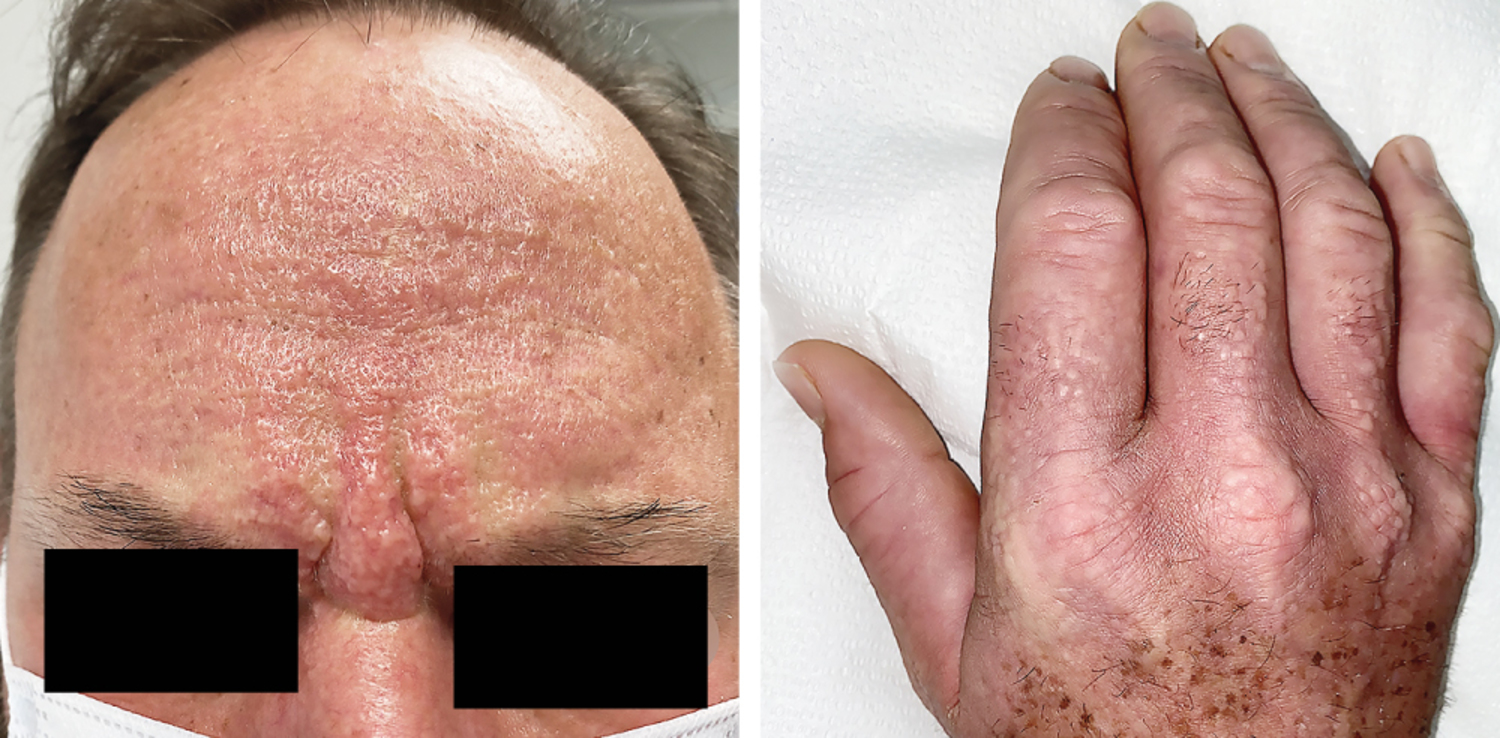
\includegraphics[width=5cm]{figs/6.png} 
%         & 
%         This is a Multi-Agent Collaborative Generation task for creating dynamic conversational interactions. 
%         Given a user query: \{user query\} and context of three distinct agents: 
%         \{Patient Agent Context\}, \{Measurement Agent Context\}, and \{Moderator Agent Context\}, 
%         Please generate a well-rounded response to the user's question.  
%         & 
%         D
%         \\
%         \hline
%         \multicolumn{1}{|c|}{\textbf{Method}} 
%         & \multicolumn{2}{c|}{\textbf{Output Results}} \\
%         \hline
%         \multicolumn{1}{|c|}{COT} 
%         & \multicolumn{2}{m{13cm}|}{\centering Based on the patient's symptoms and test results, I will go through my thought process and chain of reasoning to arrive at a diagnosis. The patient presents with a 3-year history of an itchy rash on their forehead ... This suggests that the patient may have a monoclonal gammopathy of undetermined significance (MGUS) or a plasma cell disorder. Given the patient's symptoms and test results, I believe the most likely diagnosis is: DIAGNOSIS READY: Multiple myeloma (B)} \\
%         \hline
%         \multicolumn{1}{|c|}{GWM-T} 
%         & \multicolumn{2}{m{13cm}|}{\centering D} \\
%         \hline
%     \end{tabular}
% \end{table*}
\begin{table*}[h]
    \centering
    \caption{\textbf{Multi-agent collaboration task and output comparison.} Disease-related query answering through agent interaction and external knowledge. Results show GWM-T vs COT baseline. \textbf{Note: Medical images may cause discomfort but are from real datasets.}}
    \label{tab:multiagent_collaboration}
    
    \renewcommand{\arraystretch}{1.0}
    \small % 使用小字体
    
    \begin{tabular}{|>{\centering\arraybackslash}m{4cm}|>{\centering\arraybackslash}m{5cm}|>{\centering\arraybackslash}m{5.5cm}|}
        \hline
        \multicolumn{3}{|c|}{\textbf{Task Description}} \\
        \hline
        \textbf{Task} & \multicolumn{2}{c|}{Multi-agent collaboration} \\
        \hline
        \textbf{User Query} & \textbf{Patient Agent} & \textbf{Moderator Agent} \\
        \hline
        
        53-year-old man, 3-year history: itchy rash, Raynaud's, dysphagia, burning hands. Exam: firm papules on forehead with glabellar grooves, waxy papules on hands with thickening and contractures. Similar changes on nose, lips, ears, trunk, feet. No telangiectasia/calcinosis. Sensory neuropathy in hands/arms/face. Normal thyroid. IgG-monoclonal gammopathy, normal bone marrow.
        
        Choices: (A) AL amyloidosis (B) Multiple myeloma (C) Scleredema (D) Scleromyxedema (E) Systemic sclerosis
        & 
        Role: 53-year-old patient with 3-year symptoms including itchy rash, firm forehead papules causing brow grooves, waxy hand papules with thickening and finger contractures. Experience Raynaud's phenomenon, dysphagia, burning hands, and numbness in hands/arms/face. Aware of normal thyroid tests and abnormal blood protein but unaware of diagnosis implications.
        & 
        Moderator organizing case information:
        
        Test results: Normal thyroid function, IgG-monoclonal gammopathy detected, normal bone marrow biopsy.
        
        Key findings: Extracellular yellow-brown deposits in dermis on skin biopsy.
        \\
        \hline
        \textbf{Measurement Agent} & \textbf{Action Prompt} & \textbf{Ground Truth} \\
        \hline
        \centering
        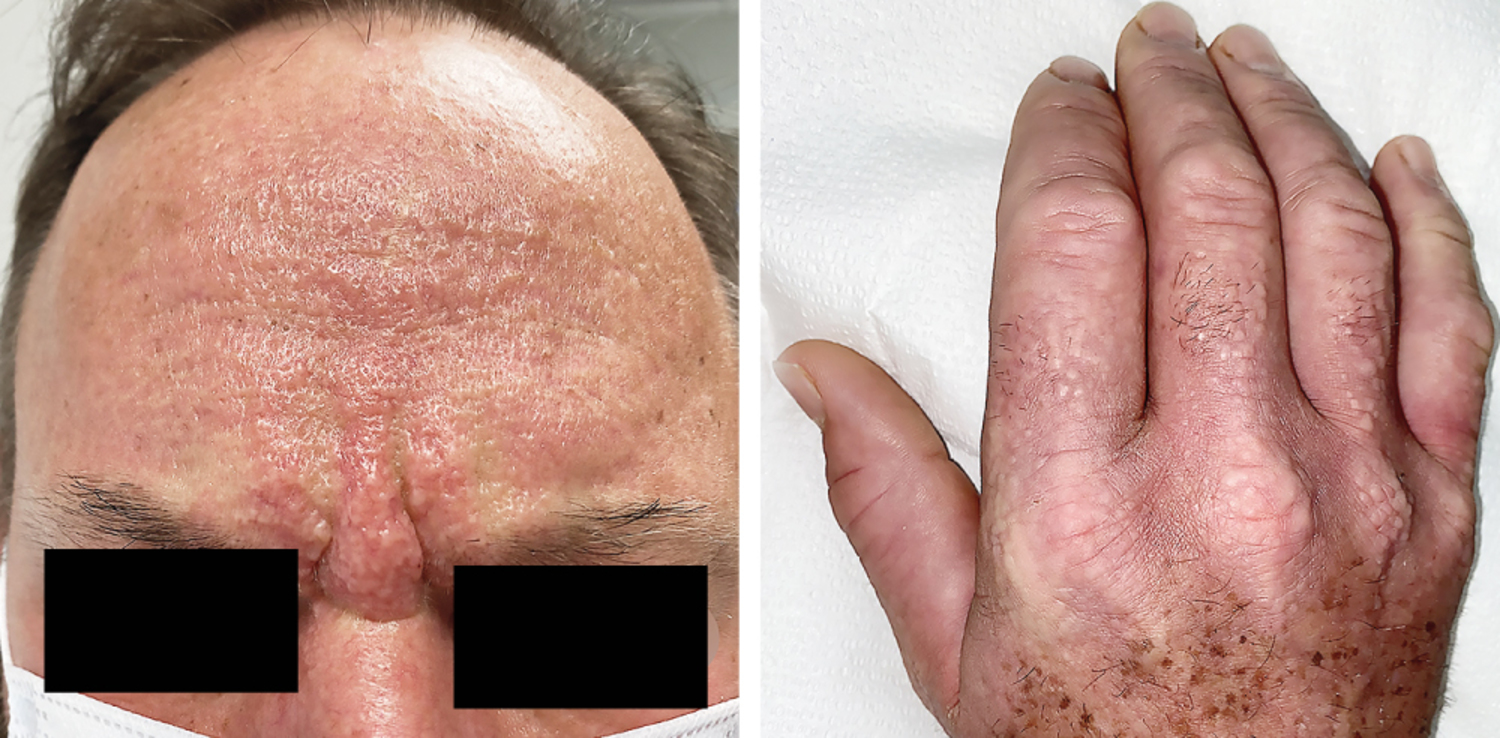
\includegraphics[width=3.5cm]{figs/6.png} 
        & 
        Multi-Agent Collaborative Generation task for dynamic conversational interactions. Generate response using Patient, Measurement, and Moderator agent contexts for the given user query.
        & 
        D
        \\
        \hline
        \textbf{Method} & \multicolumn{2}{c|}{\textbf{Output Results}} \\
        \hline
        COT & \multicolumn{2}{m{10.5cm}|}{\centering Analysis of patient symptoms and test results suggests monoclonal gammopathy with characteristic skin findings. DIAGNOSIS: Multiple myeloma (B)} \\
        \hline
        GWM-T & \multicolumn{2}{m{10.5cm}|}{\centering D} \\
        \hline
    \end{tabular}
\end{table*}
\begin{table*}[h]
    \centering
    \caption{\textbf{Task description and output comparison of retrieval-augmented generation.} This task is to generate a response that integrates information from the retrieved documents to accurately address the user's query. Here we utilize one case of LongBench v2 dataset as examples. We show the output results of GWM-E, the best performing GWM, and GPT-4o mini, the strongest baseline.}
    \label{tab:rag}
    
    \renewcommand{\arraystretch}{1.2} % Slightly increase row height
    
    % Define a new column type for centered text in m columns
    \newcolumntype{C}[1]{>{\centering\arraybackslash}m{#1}}
    
    \begin{tabular}{|C{4.5cm}|C{4.5cm}|C{4cm}|C{2cm}|C{1cm}|}
        \toprule
        \multicolumn{5}{|c|}{\textbf{Task Description}} \\
        \midrule
        \multicolumn{2}{|c|}{\textbf{Task Name}} & \multicolumn{3}{c|}{Retrieval-augmented generation} \\
        \midrule
        \textbf{User query} & \textbf{Document} & \textbf{Action prompt} & \multicolumn{2}{c|}{\textbf{Ground truth}} \\
        \midrule
        What is the correct answer to this question: You are given a grammar book of Kalamang language, now translate the following Kalamang sentence into English: Faisal emun me mindi don bolonet me ma he kademor.
Choices:
(A) Faisal's mother is still angry at him for a little thing like that.
(B) Faisal's mother turns furious at him for a big thing like that.
(C) Faisal's mother gets frustrated at him for a big thing like this.
(D) Faisal's mother gets angry at him for a little thing like that.

Format your response as follows: "The correct answer is (insert answer here)". & 
        There are very few households with two fluent Kalamang-speaking parents and children born after 1990, but even in those households the children are not raised in Kalamang. As indicated above, non-fluent speakers have a good passive command of Kalamang ... Fluent Kalamang speakers do not necessarily shift to Papuan Malay when they join the conversation, but they are not expected to actively contribute, although they can express themselves in a simple way in Kalamang ... & 
        This is a Retrieval-Augmented Generation task for improving response quality in dialogue systems. Given a user query: \{user query\} and a set of retrieved documents: \{retrieved documents\}, the goal is to generate a coherent and contextually relevant response. Please generate a response that integrates information from the retrieved documents to accurately address the user's query. & 
        \multicolumn{2}{c|}{D} \\
        \midrule
        \multicolumn{2}{|c|}{\textbf{Method}} & \multicolumn{3}{c|}{\textbf{Output Results}} \\
        \midrule
        \multicolumn{2}{|c|}{GPT-4o mini} & \multicolumn{3}{c|}{A} \\
        \midrule
        \multicolumn{2}{|c|}{GWM-E} & \multicolumn{3}{c|}{D} \\
        \bottomrule
    \end{tabular}
\end{table*}

% \begin{table*}[h]
%     \centering
%     \caption{\textbf{Task description and output comparison of planning and optimization.} This task is to predict the next decision-making behavior of the agent. We utilize one case of the ALFWorld dataset as an example, showing the output results of GWM-E, the best performing GWM, and T5 FT, the strongest baseline.}
%     \label{tab:planning_optimization}

%     \renewcommand{\arraystretch}{1.2} % Slightly increase row height

%     \begin{tabular}{|>{\centering\arraybackslash}m{4cm}|>{\centering\arraybackslash}m{3cm}|>{\centering\arraybackslash}m{5cm}|>{\centering\arraybackslash}m{0.5cm}|>{\centering\arraybackslash}m{0.5cm}|}
%         \hline
%         \multicolumn{5}{|c|}{\textbf{Task Description}} \\
%         \hline
%         \multicolumn{2}{|c|}{\textbf{Task Name}} & \multicolumn{3}{c|}{Planning and optimization} \\
%         \hline
%         \textbf{Image information} & \textbf{Text information} & \textbf{Action prompt} & \multicolumn{2}{c|}{\textbf{Ground truth}} \\
%         \hline
%         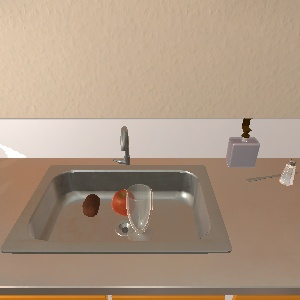
\includegraphics[width=4cm]{figs/000000000.jpg} & 
%         Your task is to: put a potato in countertop. & 
%         This is an embodied household task, please predict the next decision-making behavior based on multimodal information: \{image information\}, \{text information\}.  & 
%         \multicolumn{2}{c|}{go to garbagecan 1} \\
%         \hline
%         \multicolumn{2}{|c|}{\textbf{Method}} & \multicolumn{3}{c|}{\textbf{Output Results}} \\
%         \hline
%         \multicolumn{2}{|c|}{T5 FT} & \multicolumn{3}{m{11cm}|}{\centering go to microwave 1} \\
%         \hline
%         \multicolumn{2}{|c|}{GWM-E} & \multicolumn{3}{m{11cm}|}{\centering go to garbagecan 1} \\
%         \hline
%     \end{tabular}
% \end{table*}

\begin{table*}[h]
    \centering
    \caption{\textbf{Planning and optimization task and output comparison.} Agent decision-making prediction using ALFWorld dataset. Results show GWM-E vs T5 FT baseline.}
    \label{tab:planning_optimization}
    \renewcommand{\arraystretch}{1.0}
    \small % 使用小字体
    \begin{tabular}{|>{\centering\arraybackslash}m{3cm}|>{\centering\arraybackslash}m{2.5cm}|>{\centering\arraybackslash}m{4cm}|>{\centering\arraybackslash}m{2cm}|}
        \hline
        \multicolumn{4}{|c|}{\textbf{Task Description}} \\
        \hline
        \multicolumn{2}{|c|}{\textbf{Task}} & \multicolumn{2}{c|}{Planning and optimization} \\
        \hline
        \textbf{Image} & \textbf{Text} & \textbf{Action Prompt} & \textbf{Ground Truth} \\
        \hline
        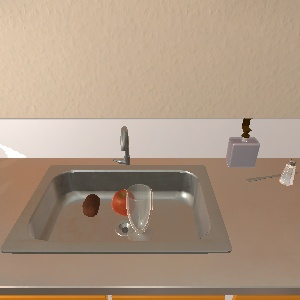
\includegraphics[width=2.8cm]{figs/000000000.jpg} & 
        Task: put a potato in countertop & 
        Embodied household task: predict next decision-making behavior based on multimodal information. & 
        go to garbagecan 1 \\
        \hline
        \multicolumn{2}{|c|}{\textbf{Method}} & \multicolumn{2}{c|}{\textbf{Output Results}} \\
        \hline
        \multicolumn{2}{|c|}{T5 FT} & \multicolumn{2}{m{6cm}|}{\centering go to microwave 1} \\
        \hline
        \multicolumn{2}{|c|}{GWM-E} & \multicolumn{2}{m{6cm}|}{\centering go to garbagecan 1} \\
        \hline
    \end{tabular}
\end{table*}

\section{Training and Inference Efficiency} \label{app:Training and Inference Efficiency}

Accurately comparing the training and inference efficiency of GWM with other FMs is highly challenging because many FMs are not designed to address multimodal problems and utilize various architectures. 
We can only compare the efficiency between GWM and LLM-based FMs from principles. For GWM-T, its efficiency shows no fundamental difference from other LLM-based FMs, as both are based on the standard instruction tuning. 
For GWM-E, its training process only requires fine-tuning the projector as stated in section \ref{sec:Projector tuning}, and its embedding-based method also saves a significant amount of token cost, making it more efficient. 
For GWM-E, it takes approximately 7 hours (\(\sim \frac{1}{4}\) of GWM-T) of training time on four NVIDIA A6000 GPUs described in implementation details of section \ref{sec:exps}, and the inference time per case averages 0.213s (similar to GWM-T).  Moreover, GWM-E significantly reduces memory usage with a shorter token length of 140.23 (\(\sim \frac{1}{14}\) of GWM-T).